\documentclass[10pt]{standalone}
\usepackage{stix}
\usepackage{tikz}
\usepackage{xcolor}
\usepackage{amsmath}
\usepackage{braket}
\definecolor{Fblue}{HTML}{560dcb}
\definecolor{Fred}{HTML}{92235a}
\definecolor{Firebrick}{HTML}{b22222}
\definecolor{Fnavy}{HTML}{000080}
\definecolor{ForangeRed}{HTML}{ff4500}
\definecolor{Fcornflower}{HTML}{bbddff}
\definecolor{Fcmix}{HTML}{0f4880}
\definecolor{Faqua}{HTML}{5fbf9f}
\newcommand{\bvec}[1]{\boldsymbol{#1}}
\usetikzlibrary{calc, arrows, arrows.meta, math}

\newcommand{\xp}[1]{\texttt{\color{ForangeRed}#1}}
\newcommand{\tp}[1]{\texttt{\color{Firebrick}#1}}
\newcommand{\tpd}[1]{\tp{#1} [displ,size]}
\newcommand{\ipd}[1]{#1 [displ, size]}

\newcommand{\bracketOne}[2]{
  \draw (cell#1.west) -- ++(-0.1,0.0) node {#2};
}
\newcommand{\bracketTwo}[3]{
  \tikzmath{\coordA = 0.5*(cell#1.west) + 0.5*(cell#2.west) + (-0.1,0.0);}
  \draw (cell#1.west) -- (\coordA);
  \draw (cell#2.west) -- (\coordA) node {#3};
}
\newcommand{\bracketThree}[4]{
  \tikzmath{\dbuf = 1./3.;
    \coordA = \dbuf*(cell#1.west) + \dbuf*(cell#2.west) + \dbuf*(cell#3.west) + (-0.1,0.0);}
  \draw (cell#1.west) -- (\coordA);
  \draw (cell#2.west) -- (\coordA);
  \draw (cell#3.west) -- (\coordA) node {#4};
}

\newcommand{\EbracketOne}[2]{
  \draw (Ecell#1.east) -- ++(0.1,0.0) node[anchor=west] {#2};
}
\newcommand{\EbracketTwo}[3]{
  \tikzmath{\coordA = 0.5*(Ecell#1.east) + 0.5*(Ecell#2.east) + (0.1,0.0);}
  \draw (Ecell#1.east) -- (\coordA);
  \draw (Ecell#2.east) -- (\coordA) node[anchor=west] {#3};
}
\newcommand{\EbracketThree}[4]{
  \tikzmath{\dbuf = 1./3.;
    \coordA = \dbuf*(Ecell#1.east) + \dbuf*(Ecell#2.east) + \dbuf*(Ecell#3.east) + (0.1,0.0);}
  \draw (Ecell#1.east) -- (\coordA);
  \draw (Ecell#2.east) -- (\coordA);
  \draw (Ecell#3.east) -- (\coordA) node[anchor=west] {#4};
}

\newcommand{\colorizeBox}[3]{
  \tikzmath{\coordA = (0,1-#1/64.0);
            \coordB = (1,1-#2/64.0);}
  \fill[draw=none, fill=#3] (\coordA) rectangle (\coordB);
}
\newcommand{\EcolorizeBox}[3]{
  \tikzmath{\coordA = (0,1-#1/64.0+67/64.0);
            \coordB = (1,1-#2/64.0+67/64.0);}
  \fill[draw=none, fill=#3] (\coordA) rectangle (\coordB);
}

\begin{document}
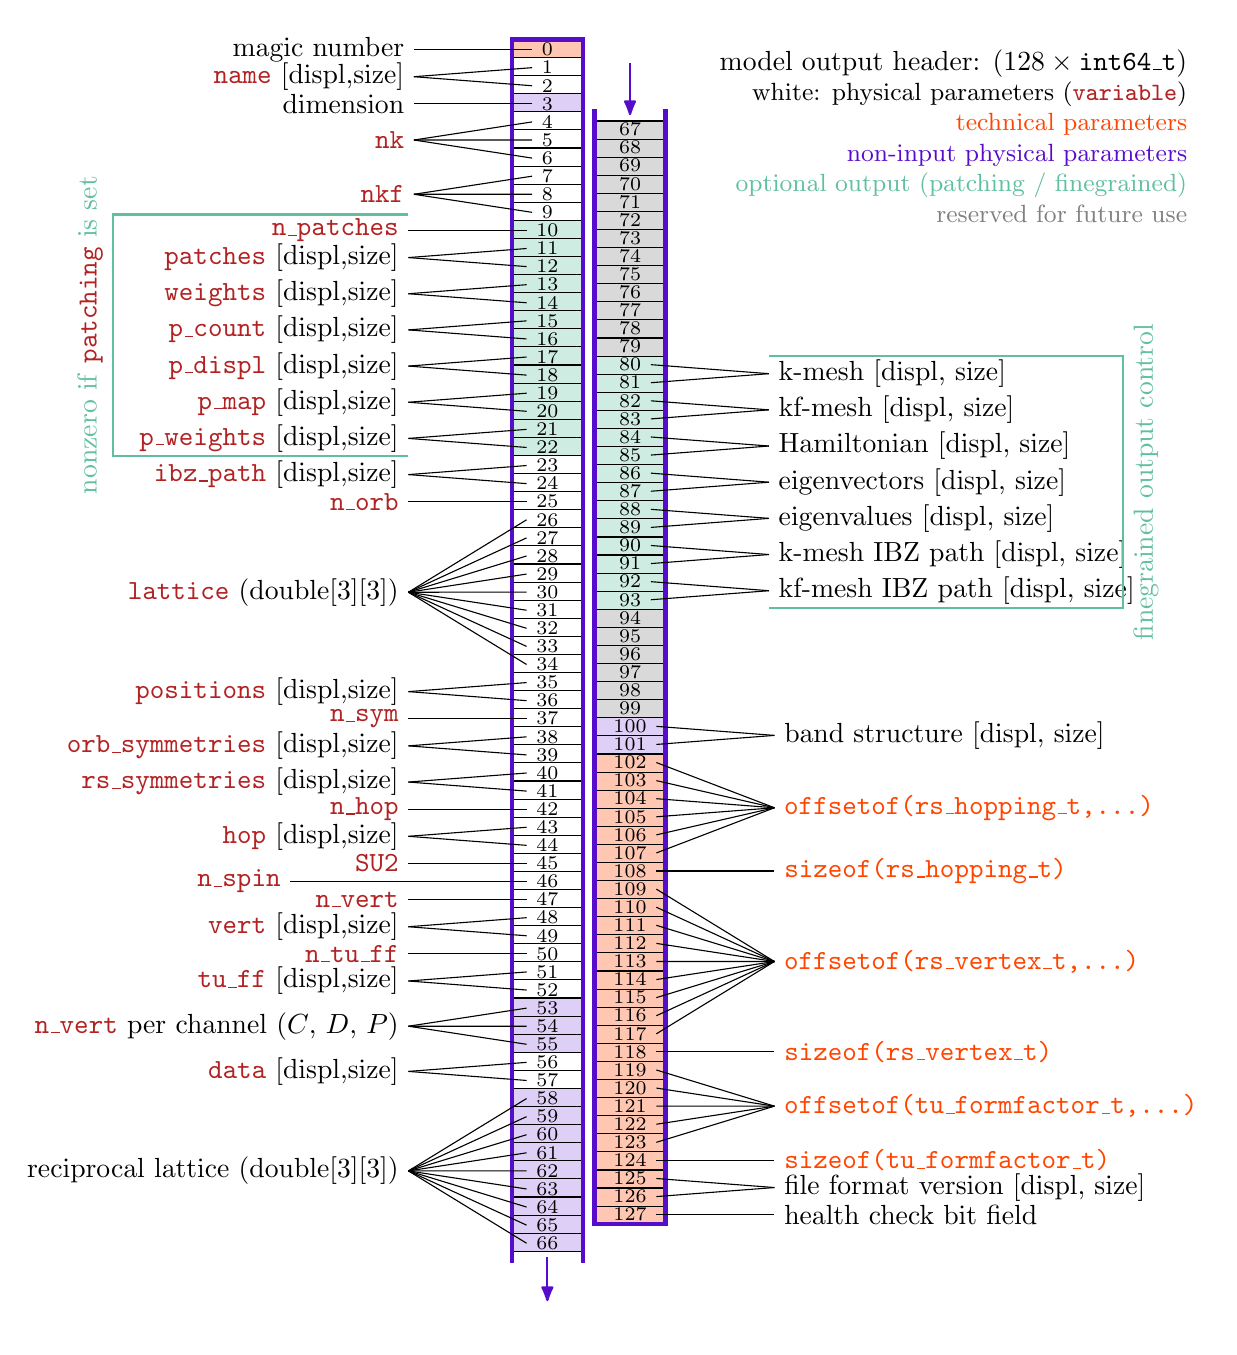
\begin{tikzpicture}[x=5.90552in, y=5.90552in, >={Latex[round]}]
  \clip (0,-0.1) rectangle (1,1.0);
  \tikzmath{
    coordinate \coordA;
    coordinate \coordB;
    int \ibuf;
    real \dbuf;
  }
  \node[anchor=north east] at (0.99,0.99) {\begin{minipage}{3in}%
    \begin{flushright}%
      model output header: $(128 \times \texttt{int64\_t})$\\
      \small
      white: physical parameters (\tp{variable}) \\
      \textcolor{ForangeRed}{technical parameters} \\
      \textcolor{Fblue}{non-input physical parameters} \\
      \textcolor{Faqua}{optional output (patching / finegrained)} \\
      \textcolor{gray}{reserved for future use}
    \end{flushright}
  \end{minipage}};

  \begin{scope}[shift={(0.41,0.01)}, yscale=0.98, xscale=0.06]
    \colorizeBox{0}{1}{ForangeRed!30!white}

    \colorizeBox{3}{4}{Fblue!20!white}
    \colorizeBox{53}{56}{Fblue!20!white}
    \colorizeBox{58}{67}{Fblue!20!white}

    \colorizeBox{10}{23}{Faqua!30!white}
    \foreach \idx in {1,2,...,67} {
      \tikzmath{
        \dbuf = 1./64.;
        \ibuf = \idx-1;
        \coordA = (0,1-\idx/64.0);
        \coordB = (1,1-\idx/64.0);
      }
      \draw (\coordA) -- node[midway, above, yshift=-0.29em] (cell\ibuf) {\scriptsize\ibuf} (\coordB);
    }
    \tikzmath{ \dbuf = -0.01 - 3./64.; }
    \draw[Fblue, ultra thick] (0,\dbuf) -- (0,1) -- (1,1) -- (1,\dbuf);
    \tikzmath{ \dbuf = -0.005 - 3./64; }
    \draw[Fblue, ->, thick] (0.5,\dbuf) -- (0.5,-0.09);
  \end{scope}
  \begin{scope}[shift={(0.48,-0.059)}, yscale=0.98, xscale=0.06]
    \EcolorizeBox{102}{128}{ForangeRed!30!white}

    \EcolorizeBox{100}{102}{Fblue!20!white}

    \EcolorizeBox{80}{94}{Faqua!30!white}

    \EcolorizeBox{67}{80}{gray!30!white}
    \EcolorizeBox{94}{100}{gray!30!white}

    \foreach \idx in {0,1,...,60} {
      \tikzmath{
        \dbuf = 1./64.;
        \ibuf = \idx+67;
        \coordA = (0,1-\idx/64.0);
        \coordB = (1,1-\idx/64.0);
      }
      \draw (\coordA) -- node[midway, below, yshift=0.27em] (Ecell\ibuf) {\scriptsize\ibuf} (\coordB);
    }
    \tikzmath{\dbuf = 1.0 - 61.0/64.0;}
    \draw[Fblue, ultra thick] (0,1.01) -- (0,\dbuf) -- (1,\dbuf) -- (1,1.01);
    \draw[Fblue, ->, thick] (0.5,1.05) -- (0.5,1.005);
  \end{scope}
  \begin{scope}[anchor=east]
    \bracketOne{0}{magic number}
    \bracketTwo{1}{2}{\tpd{name}}
    \bracketOne{3}{dimension}
    \bracketThree{4}{5}{6}{\tp{nk}}
    \bracketThree{7}{8}{9}{\tp{nkf}}

    \bracketOne{10}{\tp{n\_patches}}
    \bracketTwo{11}{12}{\tpd{patches}}
    \bracketTwo{13}{14}{\tpd{weights}}
    \bracketTwo{15}{16}{\tpd{p\_count}}
    \bracketTwo{17}{18}{\tpd{p\_displ}}
    \bracketTwo{19}{20}{\tpd{p\_map}}
    \bracketTwo{21}{22}{\tpd{p\_weights}}
    \tikzmath{\coordA = (cell10.north west) + (-0.1,0);
              \coordB = (cell22.west) + (-0.1,-0.007);}
    \tikzmath{coordinate \cbufA;
              coordinate \cbufB;
              \cbufA = (\coordA) + (-0.25,0);
              \cbufB = (\coordB) + (-0.25,0);}
    \draw[Faqua, thick] (\coordA) -- (\cbufA) -- node[midway, above, rotate=90]{nonzero if \tp{patching} is set} (\cbufB) -- (\coordB);

    \bracketTwo{23}{24}{\tpd{ibz\_path}}
    \bracketOne{25}{\tp{n\_orb}}

    \tikzmath{\dbuf=1./9.;
      \coordA = \dbuf*(cell26.west) +
                \dbuf*(cell27.west) +
                \dbuf*(cell28.west) +
                \dbuf*(cell29.west) +
                \dbuf*(cell30.west) +
                \dbuf*(cell31.west) +
                \dbuf*(cell32.west) +
                \dbuf*(cell33.west) +
                \dbuf*(cell34.west) + (-0.1,0.0);}
    \draw (cell26.west) -- (\coordA);
    \draw (cell27.west) -- (\coordA);
    \draw (cell28.west) -- (\coordA);
    \draw (cell29.west) -- (\coordA);
    \draw (cell30.west) -- (\coordA);
    \draw (cell31.west) -- (\coordA);
    \draw (cell32.west) -- (\coordA);
    \draw (cell33.west) -- (\coordA);
    \draw (cell34.west) -- (\coordA) node {\tp{lattice} (double[3][3])};

    \bracketTwo{35}{36}{\tpd{positions}}
    \bracketOne{37}{\tp{n\_sym}}
    \bracketTwo{38}{39}{\tpd{orb\_symmetries}}
    \bracketTwo{40}{41}{\tpd{rs\_symmetries}}
    \bracketOne{42}{\tp{n\_hop}}
    \bracketTwo{43}{44}{\tpd{hop}}
    \bracketOne{45}{\tp{SU2}}
    \draw (cell46.west) -- ++(-0.2,0.0) node {\tp{n\_spin}};
    \bracketOne{47}{\tp{n\_vert}}
    \bracketTwo{48}{49}{\tpd{vert}}
    \bracketOne{50}{\tp{n\_tu\_ff}}
    \bracketTwo{51}{52}{\tpd{tu\_ff}}
    \bracketThree{53}{54}{55}{\tp{n\_vert} per channel ($C$, $D$, $P$)}
    \bracketTwo{56}{57}{\tpd{data}}

    \tikzmath{\dbuf=1./9.;
      \coordA = \dbuf*(cell58.west) +
                \dbuf*(cell59.west) +
                \dbuf*(cell60.west) +
                \dbuf*(cell61.west) +
                \dbuf*(cell62.west) +
                \dbuf*(cell63.west) +
                \dbuf*(cell64.west) +
                \dbuf*(cell65.west) +
                \dbuf*(cell66.west) + (-0.1,0.0);}
    \draw (cell58.west) -- (\coordA);
    \draw (cell59.west) -- (\coordA);
    \draw (cell60.west) -- (\coordA);
    \draw (cell61.west) -- (\coordA);
    \draw (cell62.west) -- (\coordA);
    \draw (cell63.west) -- (\coordA);
    \draw (cell64.west) -- (\coordA);
    \draw (cell65.west) -- (\coordA);
    \draw (cell66.west) -- (\coordA) node {reciprocal lattice (double[3][3])};

    \EbracketTwo{80}{81}{\ipd{k-mesh}}
    \EbracketTwo{82}{83}{\ipd{kf-mesh}}
    \EbracketTwo{84}{85}{\ipd{Hamiltonian}}
    \EbracketTwo{86}{87}{\ipd{eigenvectors}}
    \EbracketTwo{88}{89}{\ipd{eigenvalues}}
    \EbracketTwo{90}{91}{\ipd{k-mesh IBZ path}}
    \EbracketTwo{92}{93}{\ipd{kf-mesh IBZ path}}
    \tikzmath{\coordA = (Ecell80.east) + (0.1,0.007);
              \coordB = (Ecell93.east) + (0.1,-0.007);}
    \tikzmath{coordinate \cbufA;
              coordinate \cbufB;
              \cbufA = (\coordA) + (0.3,0);
              \cbufB = (\coordB) + (0.3,0);}
    \draw[Faqua, thick] (\coordA) -- (\cbufA) -- node[midway, below, rotate=90]{
      finegrained output control} (\cbufB) -- (\coordB);

    \EbracketTwo{100}{101}{\ipd{band structure}}

    \tikzmath{\dbuf=1./6.;
      \coordA = \dbuf*(Ecell102.east) +
                \dbuf*(Ecell103.east) +
                \dbuf*(Ecell104.east) +
                \dbuf*(Ecell105.east) +
                \dbuf*(Ecell106.east) +
                \dbuf*(Ecell107.east) + (0.1,0.0);}
    \draw (Ecell102.east) -- (\coordA);
    \draw (Ecell103.east) -- (\coordA);
    \draw (Ecell104.east) -- (\coordA);
    \draw (Ecell105.east) -- (\coordA);
    \draw (Ecell106.east) -- (\coordA);
    \draw (Ecell107.east) -- (\coordA) node[anchor=west] {\xp{offsetof(rs\_hopping\_t,...)}};
    \EbracketOne{108}{\xp{sizeof(rs\_hopping\_t)}}

    \tikzmath{\dbuf=1./9.;
      \coordA = \dbuf*(Ecell109.east) +
                \dbuf*(Ecell110.east) +
                \dbuf*(Ecell111.east) +
                \dbuf*(Ecell112.east) +
                \dbuf*(Ecell113.east) +
                \dbuf*(Ecell114.east) +
                \dbuf*(Ecell115.east) +
                \dbuf*(Ecell116.east) +
                \dbuf*(Ecell117.east) + (0.1,0.0);}
    \draw (Ecell109.east) -- (\coordA);
    \draw (Ecell110.east) -- (\coordA);
    \draw (Ecell111.east) -- (\coordA);
    \draw (Ecell112.east) -- (\coordA);
    \draw (Ecell113.east) -- (\coordA);
    \draw (Ecell114.east) -- (\coordA);
    \draw (Ecell115.east) -- (\coordA);
    \draw (Ecell116.east) -- (\coordA);
    \draw (Ecell117.east) -- (\coordA) node[anchor=west] {\xp{offsetof(rs\_vertex\_t,...)}};
    \EbracketOne{118}{\xp{sizeof(rs\_vertex\_t)}}

    \tikzmath{\dbuf=1./5.;
      \coordA = \dbuf*(Ecell119.east) +
                \dbuf*(Ecell120.east) +
                \dbuf*(Ecell121.east) +
                \dbuf*(Ecell122.east) +
                \dbuf*(Ecell123.east) + (0.1,0.0);}
    \draw (Ecell119.east) -- (\coordA);
    \draw (Ecell120.east) -- (\coordA);
    \draw (Ecell121.east) -- (\coordA);
    \draw (Ecell122.east) -- (\coordA);
    \draw (Ecell123.east) -- (\coordA) node[anchor=west] {\xp{offsetof(tu\_formfactor\_t,...)}};
    \EbracketOne{124}{\xp{sizeof(tu\_formfactor\_t)}}

    \EbracketTwo{125}{126}{\ipd{file format version}}
    \EbracketOne{127}{health check bit field}

    \tikzmath{\coordA = 0.5*(Ecell67.east) + 0.5*(Ecell79.east) + (0.1,0.0);
              \coordB = 0.5*(Ecell94.east) + 0.5*(Ecell99.east) + (0.1,0.0);}
  \end{scope}
\end{tikzpicture}
\end{document}

